\subsection{Examples}

\begin{example2}{CPU Components}\\
Nennen Sie die Hauptkomponenten der M0 CPU und erklären Sie ihre Funktion:
\begin{itemize}
  \item \textbf{Core Registers}:
    \begin{itemize}
      \item 13 x 32-bit Register für temporäre Speicherung (R0 – R12)
      \item 1 x 32-bit Register für Stack Pointer (SP) (R13)
      \item 1 x 32-bit Register für Link Register (LR) (R14)
      \item 1 x 32-bit Register für Program Counter (PC) (R15)
    \end{itemize}
  \item \textbf{ALU} (Arithmetic Logic Unit):
    \begin{itemize}
      \item Data processing unit for arithmetic and logic operations
    \end{itemize}
  \item \textbf{Flags}:
    \begin{itemize}
      \item Processor Status Register: Indicates the state of the processor
    \end{itemize}
  \item \textbf{Control Unit with Instruction Register}:
    \begin{itemize}
      \item Controls execution of an instruction based on the machine code currently stored in the Instruction Register (IR)
    \end{itemize}
  \item \textbf{Bus Interface}:
    \begin{itemize}
      \item Interface between CPU and external System Bus
      \item Bridge between internal and external bus
    \end{itemize}
\end{itemize}
\end{example2}

\begin{example2}{Special Purpose Registers}\\
Beschreiben Sie die Funktion folgender Register:
\begin{itemize}
  \item \textbf{PC (Program Counter)}:
    \begin{itemize}
      \item Points to the address where the instructions will next be read
    \end{itemize}
  \item \textbf{SP (Stack Pointer)}:
    \begin{itemize}
      \item Points to the memory addresses where the elements are written/read from the stack
    \end{itemize}
  \item \textbf{LR (Link Register)}:
    \begin{itemize}
      \item Used to keep track of the positions where to jump back (e.g. routines)
    \end{itemize}
\end{itemize}
\end{example2}

\begin{example2}{Program Counter Initialization}\\
Warum wird der PC bei Reset auf einen definierten Wert initialisiert (während andere CPU Register undefinierte Werte haben können)?\\
So that fetching of the first instruction can always start at the same (known and predictable) place.
\end{example2}

\begin{example2}{M0 Instruction Types}\\
Name 3 instruction types of the M0 CPU:
\begin{itemize}
  \item Data transfer
  \item Data processing
  \item Flow control
\end{itemize}
\end{example2}

\begin{example2}{Instruction Execution Analogy}\\
Ein Prozessor führt eine Liste von Instruktionen in einer vordefinierten Reihenfolge aus. Finden Sie Analogien aus dem Alltag:
\begin{itemize}
  \item Baker/Koch, der einem Rezept folgt
  \item Musiker, der nach Noten spielt
  \item Pilot, der vor dem Start eine Checkliste durchgeht
\end{itemize}
\end{example2}







\begin{example2}{Assembly Code Structure}\\
Name the different parts of a line in assembly code:
\begin{lstlisting}[language=armasm, style=basesmol]
label   MOVS    R0, #42     ; This is a comment
\end{lstlisting}
Components:
\begin{itemize}
  \item Label
  \item Mnemonic (instruction)
  \item Operands
  \item Comment
\end{itemize}
\end{example2}

\begin{example2}{Terms in Memory}
Explain the following terms:
\begin{itemize}
  \item \textbf{Fetch}: Get the instruction from code memory
  \item \textbf{Execute}: Do what the instructions say
  \item \textbf{Word}: A 32-bit memory unit (for the MO)
  \item \textbf{Half-word}: A 16-bit memory unit (for the MO)
  \item \textbf{Little endian}: A multi-byte representation where the LSByte is at the lower address
  \item \textbf{Big endian}: A multi-byte representation where the MSByte is at the lower address
  \item \textbf{Word Alignment}: The address of the multi-byte element is a multiple of the word length (4 for the MO)
  \item \textbf{Data transfer}: Move data between registers and memory
  \item \textbf{Data processing}: Perform arithmetic and logic operations
  \item \textbf{Flow control}: Change the order of execution
  \item \textbf{Stack}: Memory area for procedure calls and local variables
  \item \textbf{Heap}: Memory area for dynamic memory allocation
  \item \textbf{Global variables}: Variables accessible from all functions
  \item \textbf{Local variables}: Variables accessible only within a function
  \item \textbf{Static variables}: Variables with fixed memory allocation
  \item \textbf{Constants}: Fixed values used in the program
  \item \textbf{Code section}: Memory area for instructions
  \item \textbf{Data section}: Memory area for variables
  \item \textbf{Stack section}: Memory area for runtime data
  \item \textbf{Memory map}: Graphical layout showing addresses and sizes of elements
  \item \textbf{Memory areas}: Sections of memory for different purposes
  \item \textbf{Memory sections}: Organized parts of memory for program use
  \item \textbf{Memory ranges}: Address ranges for different memory sections
\end{itemize}
\end{example2}

\columnbreak

\begin{example2}{Memory Map Usage}\\
What is a memory map? What is it used for?
\begin{itemize}
  \item It is a graphical layout (map) showing the addresses and sizes of elements that communicate with the CPU (memories, Inputs, Outputs)
  \item The memory map helps users to know where each element is (e.g. when writing the appropriate drivers)
\end{itemize}
\end{example2}


\begin{example2}{Memory Areas}\\
Which 3 memory areas (sections) can be differentiated for a program?

\begin{itemize}
  \item \textbf{CODE} (read-only $\rightarrow$ RAM or ROM):
    \begin{itemize}
      \item Machine instructions
      \item Constants
    \end{itemize}
  \item \textbf{DATA} (read-write $\rightarrow$ RAM):
    \begin{itemize}
      \item Global variables
      \item Static variables
      \item Heap in C
    \end{itemize}
  \item \textbf{STACK} (read-write $\rightarrow$ RAM):
    \begin{itemize}
      \item Procedure calls
      \item Passing of parameters
      \item Local variables
    \end{itemize}
\end{itemize}
\end{example2}

\begin{example2}{Memory Areas/Memory Map}\\
Assume that the following memory areas are used when executing a program:

\begin{itemize}
  \item Code: $0 \times 20000000$ to $0 x 200001 F F$
  \item Data: 0x20000200 to 0x200002FF
  \item Stack: 0x20000300 to 0x200003FF
\end{itemize}

Draw an appropriate memory map and draw the three sections. Label the first and last addresses for each area. How many storage locations does each of the areas contain?\\

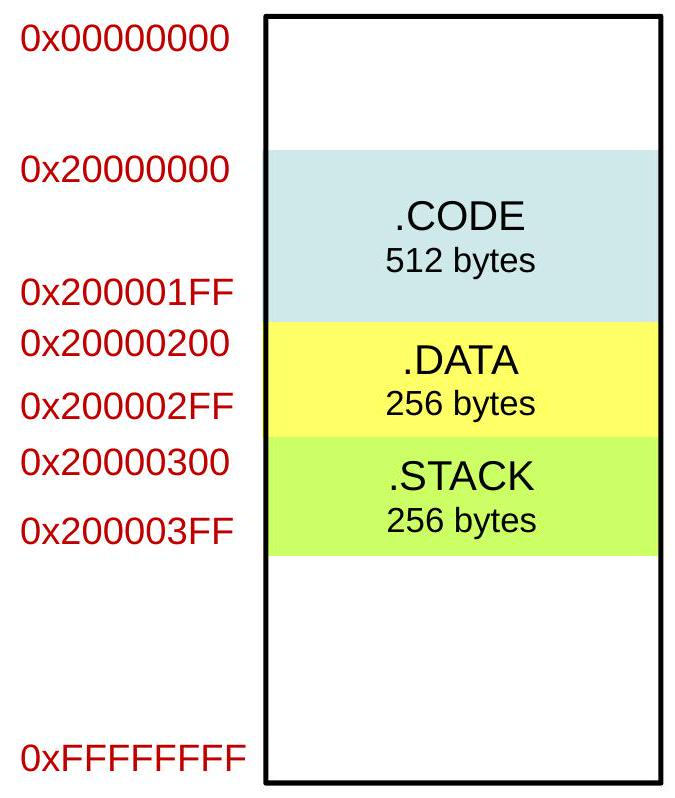
\includegraphics[width=0.6\linewidth]{images/2025_01_02_5d04f07cd96c1366bf1bg-5}
\end{example2}

\begin{KR}{Memory Section Organization}\\
Guidelines for organizing program memory sections:

1. Determine required sections:
\begin{itemize}
  \item Code section for instructions
  \item Data section for variables
  \item Stack section for runtime data
\end{itemize}

2. Calculate section sizes:
\begin{itemize}
  \item Add up all code space needs
  \item Account for all global/static variables
  \item Estimate maximum stack depth
\end{itemize}

3. Assign memory ranges:
\begin{lstlisting}[language=armasm, style=basesmol]
AREA    |.text|, CODE, READONLY
; Code section starts here

AREA    |.data|, DATA, READWRITE
; Data section starts here

; Stack section typically defined in startup code
Stack_Size    EQU     0x400    ; 1KB
AREA    STACK, NOINIT, READWRITE, ALIGN=3
Stack_Mem    SPACE    Stack_Size
\end{lstlisting}
\end{KR}




\begin{example2}{Memory Addressing}\\
Wie viele Memory Bytes können mit verschiedenen Adressbreiten adressiert werden?
\begin{itemize}
  \item 8 bit $\rightarrow$ 256 Bytes ($2^8$)
  \item 16 bit $\rightarrow$ 64 KBytes = 65'536 Bytes ($2^{16}$)
  \item 32 bit $\rightarrow$ 4 GBytes = 4'294'967'296 Bytes ($2^{32}$)
\end{itemize}
\end{example2}



\begin{example2}{Memory addressing}\\
How many byte positions can be addressed by the M0? Which positions in the memory map need to be occupied? Explain your answer.
\vspace{2mm}\\
The M0 has a 32-Bit address bus. Therefore, it can address 4 GByte $=2^{32}$ Bytes. Positions needed for the initialization of the processor (at Boot) must be covered by the proper elements (memory). Otherwise, there will be no correct start.\\
\end{example2}

\begin{example2}{Memory Values Example}\\
A program has variables represented as below in the memory map. Determine the decimal values assuming Little Endian representation:

\begin{tabular}{|l|l|l|}
\hline
Address & Byte content & Variable \\
\hline
0x2FFF´FFF8 & 0xE2 & Var4 (16-bit short) \\
0x2FFF´FFF9 & 01100010 (binary) & \\
\hline
0x2FFF´FFFC & 0x65 & Var3 (32-bit unsigned) \\
0x2FFF´FFFD & 10101101 & \\
0x2FFF´FFFE & 0xA3 & \\
0x2FFF´FFFF & 0x82 & \\
\hline
\end{tabular}

Solutions:
\begin{itemize}
  \item Var4 = 0x62E2 = +25'314d (16-bit signed)
  \item Var3 = 0x82A3AD65 = +2'191'764'837d (32-bit unsigned)
\end{itemize}
\end{example2}



\begin{example2}{Little Endian vs. Big Endian}\\
A program (code in C) has variables represented as below in the memory map. Determine the decimal values of the variables Var1 .... Var5. Assume Little Endian representation.
\begin{center}
\begin{tabular}{|c|c|c|}
\hline
Address & Byte content  & Variable \\
& (decimal, hex, binary) & \\
\hline
0x2FFF'FFF7 & 0x45 &  \\
\hline
0x2FFF'FFF8 & 0xE2 & Var4 (16-bit short) \\
\hline
0x2FFF'FFF9 & 01100010 (binary) &  \\
\hline
0x2FFF'FFFA & 213 &  \\
\hline
0x2FFF'FFFB & 25 &  \\
\hline
0x2FFF'FFFC & 0x65 & Var3 (32-bit  \\
& & unsigned integer) \\
\hline
0x2FFF'FFFD & 10101101(binary) &  \\
\hline
0x2FFF'FFFE & 0xA3 &  \\
\hline
0x2FFF'FFFF & 0x82 &  \\
\hline
0x3000'0000 & 0xA2 & Var5 (32-bit integer) \\
\hline
0x3000'0001 & 34 &  \\
\hline
0x3000'0002 & 0x54 &  \\
\hline
0x3000'0003 & 0xFF &  \\
\hline
0x3000'0004 & 0x92 & Var2 (unsigned char) \\
\hline
$0 \times 3000{ }^{\prime} 0005$ & 0x03 & Var1 (char) \\
\hline
\end{tabular}
\end{center}
Var1 $=0 \times 03=3 d$ (it is 8-bit unsigned)

Var2 $=0 \times 92=146 \mathrm{~d}$ (it is 8 -bit unsigned)

Var3 $=0 \times 82 A 3 A D 65=+2^{\prime} 191^{\prime} 764$ '837d (it is 32-bit unsigned!!)

Var4 $=0 \times 62 \mathrm{E} 2=+25$ '314d (it is 16 -bit signed)

Var5 $=0 x F F 5422 A 2=-1^{\prime} 1263$ '326 (it is 32-bit signed)\\
(-2'147'483'648 + 2'136'220'322)
\vspace{2mm}\\
How would the same variable values be stored on a Big Endian platform? Fill in the table.
\begin{center}
\begin{tabular}{|c|c|c|}
\hline
Address & Byte content & Variable \\
& (decimal, hex, binary) & \\
\hline
0x2FFF'FFF7 & 0x45 &  \\
\hline
0x2FFF'FFF8 & 01100010 (binary) & Var4 (short) \\
\hline
0x2FFF'FFF9 & 0xE2 &  \\
\hline
0x2FFF'FFFA & 213 (or 25) &  \\
\hline
0x2FFF'FFFB & 25 (or 213) &  \\
\hline
0x2FFF'FFFC & 0x82 & Var3 (32-bit  \\
& & unsigned integer) \\
\hline
0x2FFF'FFFD & 0xA3 &  \\
\hline
0x2FFF'FFFE & 10101101(binary) &  \\
\hline
0x2FFF'FFFF & $0 \times 65$ &  \\
\hline
0x3000'0000 & 0xFF & Var5 (32-bit integer) \\
\hline
0x3000'0001 & 0x54 &  \\
\hline
0x3000'0002 & 34 &  \\
\hline
0x3000'0003 & 0xA2 &  \\
\hline
0x3000'0004 & $0 \times 92$ & Var2 (unsigned char) \\
\hline
0x3000'0005 & $0 \times 03$ & Var1 (char) \\
\hline
\end{tabular}
\end{center}
We are not told if 25 / 213 form a unit or not. Therefore, it can be both ways.
\end{example2}


\begin{KR}{Calculating Memory Usage in Assembly}

1. Code Section (ROM/Flash) Calculation:
\begin{lstlisting}[language=armasm, style=basesmol]
; Each instruction is either:
; - 16 bits (2 bytes) for Thumb instructions
; - 32 bits (4 bytes) for special cases

; Example calculation:
MOVS    R0, #42         ; 2 bytes (16-bit instruction)
LDR     R0, =0x1234     ; 2 bytes + 4 bytes literal
ADDS    R0, R1          ; 2 bytes
BX      LR              ; 2 bytes
------------------------------------
Total code:             12 bytes
\end{lstlisting}

2. Data Section (RAM) Calculation:
\begin{lstlisting}[language=armasm, style=basesmol]
; Data directives memory usage:
var1    DCB     0x42        ; 1 byte
var2    DCW     0x1234      ; 2 bytes
var3    DCD     0x12345678  ; 4 bytes
array1  SPACE   10          ; 10 bytes
string1 DCB     "Hello",0   ; 6 bytes (including null)
        ALIGN   4           ; 2 padding bytes
------------------------------------
Total data:                 25 bytes
\end{lstlisting}

3. Common Memory Units:
\begin{itemize}
  \item \textbf{DCB} (Define Constant Byte): 1 byte per value
  \item \textbf{DCW} (Define Constant HalfWord): 2 bytes per value
  \item \textbf{DCD} (Define Constant Word): 4 bytes per value
  \item \textbf{SPACE}: Reserves specified number of bytes
  \item \textbf{ALIGN}: Adds padding bytes for alignment
\end{itemize}

4. Stack Usage Calculation:
\begin{lstlisting}[language=armasm, style=basesmol]
my_function
    PUSH    {R4-R7, LR}     ; 5 registers * 4 bytes = 20 bytes
    SUB     SP, SP, #16     ; Local array = 16 bytes
    ; ... function body ...
    ADD     SP, SP, #16     ; Deallocate array
    POP     {R4-R7, PC}     ; Restore 20 bytes
------------------------------------
Maximum stack usage:         36 bytes
\end{lstlisting}
\end{KR}

\columnbreak

\begin{concept}{Memory Calculation Checklist}
\begin{itemize}
  \item \textbf{Code Memory}:
    \begin{itemize}
      \item Count instructions (mostly 2 bytes each)
      \item Add literal pool entries (4 bytes each)
      \item Include alignment padding
    \end{itemize}
  \item \textbf{Static Data}:
    \begin{itemize}
      \item Sum all DCB/DCW/DCD/SPACE directives
      \item Account for string terminators
      \item Include alignment requirements
    \end{itemize}
  \item \textbf{Stack Memory}:
    \begin{itemize}
      \item Count PUSH/POP register pairs
      \item Add local variable allocations
      \item Consider nested function calls
    \end{itemize}
\end{itemize}
\end{concept}

\begin{example2}{Memory Usage Calculation}
\begin{lstlisting}[language=armasm, style=basesmol]
    AREA    |.text|, CODE, READONLY
    EXPORT  process_data
    
process_data                 ; Code memory:
    PUSH    {R4,LR}         ; 2 bytes
    LDR     R0, =data_buf   ; 2 + 4 bytes (literal)
    MOVS    R1, #10         ; 2 bytes
    BL      helper_func     ; 2 bytes
    POP     {R4,PC}         ; 2 bytes

    AREA    |.data|, DATA, READWRITE
data_buf    SPACE   20      ; Data memory: 20 bytes
count       DCD     0       ; Data memory: 4 bytes
            ALIGN   4       ; Padding: 0 bytes

Total Memory Usage:
Code:   14 bytes (ROM)
Data:   24 bytes (RAM)
Stack:  8 bytes (temporary)
\end{lstlisting}
\end{example2}



